% \section{Information Theory}
Information theory provides us the tools to study the information processing capabilities of different systems. These systems include computers, artificial intelligence and also the brain. The story of Information Theory begins with Shannon who provided the tools to estimate information \cite{shin1949mathematical}. The most fundamental aspect of information theory is the concept of the 'bit'. 

As a standard, information theory deals with 'bits'. One bit of information represents a choice between two equally probable options. A perfectly balanced coin toss contains one bit of information. It has 50\% chance of landing on heads and 50\% chance of landing on tails. A bit is a measure of information and a measure of uncertainty. Thus uncertainty and information are tightly intertwined. If we are completely certain about a certain event, there is no information to be gained. 

This chapter will cover the most important aspects of information theory. First and foremost, this means discussing entropy. Once we have an understanding of entropy, extensions can be discussed. These include joint entropy and conditional entropy. With these tools, we can go into the area of mutual information, which plays an important role in this thesis. Another important aspect is the generalisation into multivariate systems and dealing with continuous (as opposed to discrete) systems. Finally, some explanation is provided of coding theory and cybernetics.

\section{Entropy}

The next step is entropy. There are different kinds of entropy, such as thermodynamic entropy. Here, we are talking about information entropy. Information entropy is the average uncertainty associated with a random variable. In other words, information entropy is the average rate of information from a random or stochastic variable. 

In order to calculate the entropy, we require some discrete random variable X, with ${x_1 ... x_n}$ the different values from X. $P(x)$ is the probability mass function. The entropy $H(X)$ can be calculated as:

\begin{equation}
H(X) = -\sum_{i=1}^{n}P(x_i)log_2(P(x_i))
\end{equation}

Interesting to note is that $log_2(P(x_i))$ is the information about value $x_i$. This formula can be extended into the conditional entropy of two events $X$ and $Y$. The entropy $H(X|Y)$ is the entropy of random variable X given that the outcome of Y is known.

\begin{equation}
H(X|Y) = \sum_{i,j}P(x_i, y_j)log_2(\frac{P(y_j)}{P(x_i, y_j)}) = -\sum_{i,j}P(x_i, y_j)log_2(\frac{P(x_i, y_j)}{P(y_j)})
\end{equation}

If random variables X and Y are independent of each other, then $H(X|Y) = H(X)$. If the variables are completely independent, knowing anything about Y, will not change anything we know about X. Similarly, if $H(X|Y) = 0$, then X is completely determined by Y. 

The rule of Bayes is also applicable to conditional entropy:

\begin{equation}
H(X|Y) = H(Y|X) + H(X) - H(Y)
\end{equation}

\section{Joint Entropy}

$H(X)$ and $H(X|Y)$ are basic notions of information measures. Figure~\ref{entropy} visualises the notion of entropy. This figure also contains two information measures that are not yet described, $I(X,Y)$ and $H(X,Y)$. Respectively, they are the mutual information and the joint entropy.

\begin{figure}[!htb]
\caption{Venn diagram for information measures.}
\label{entropy}
    \centering
    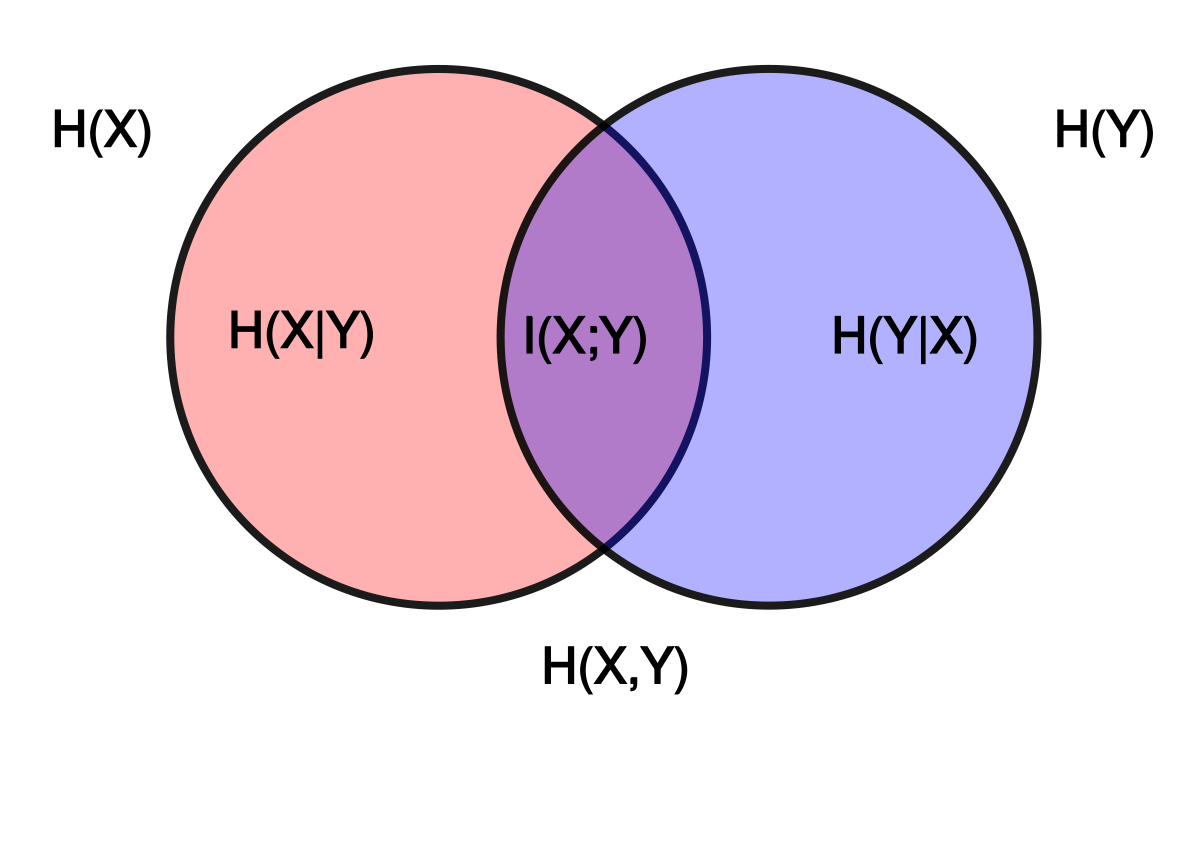
\includegraphics[width=0.8\textwidth]{fig/entropy}
\end{figure}

In the figure, $H(X,Y)$ is the complete information content of X and Y. Using the following equation, we can calculate $H(X,Y)$:

\begin{equation}
H(X,Y) = -\sum_{i=1}^{n}\sum_{j=1}^{m}P(x_i, y_j)log_2(P(x_i, y_j))
\end{equation}

Using figure~\ref{entropy}, we can see some interesting relations. $H(X,Y)$ is related to $H(X|Y)$ and $H(X)$:
\begin{equation}\label{joint}
H(X,Y) = H(X|Y) + H(Y)
\end{equation}

This can be validated:
\begin{align*}
H(X,Y) &= -\sum_{i=1}^{n}\sum_{j=1}^{m}P(x_i, y_j)log_2(P(x_i, y_j))\\
&= -\sum_{i=1}^{n}\sum_{j=1}^{m}P(x_i, y_j)log_2(P(y_i)P(x_i | y_j))\\
&= -\sum_{i=1}^{n}\sum_{j=1}^{m}P(x_i, y_j)log_2(P(y_i))-\sum_{i=1}^{n}\sum_{j=1}^{m}P(x_i, y_j)log_2(P(x_i | y_j))\\
&= -\sum_{j=1}^{m}P(y_j)log_2(P(y_i))-\sum_{i=1}^{n}\sum_{j=1}^{m}P(x_i, y_j)log_2(P(x_i | y_j))\\
&= H(Y) + H(X|Y)
\end{align*}

This relation is useful for the actual implementation of information theoretical algorithms. An important note about entropy, conditional entropy and joint entropy is that they are non-negative. It would not make sense for a random variable to have a negative information content. Joint entropy is also always greater or equal to individual entropy and joint entropy is smaller or equal to the sum of individual entropies.

\begin{equation}
H(X) \ge 0
\end{equation}

\begin{equation}
H(X|Y) \ge 0
\end{equation}

\begin{equation}
H(X,Y) \ge 0
\end{equation}

\begin{equation}
H(X,Y) \ge H(X)
\end{equation}

\begin{equation}
H(X,Y) \le H(X) + H(Y) 
\end{equation}

\section{Mutual Information}
Mutual information is the amount of information that is common between two variables. Figure~\ref{entropy} shows the mutual information as the intersection between $H(X)$ and $H(Y)$. This can also be seen in figure~\ref{mutual}. The figure also shows how mutual information can be computed. The individual entropies are summed and the joint entropy is subtracted. Another equal interpretation of mutual information is that mutual information measures the reduction in uncertainty or information when we observe one of the variables.

\begin{figure}[!htb]
\caption{Venn diagram for mutual information.}
\label{mutual}
    \centering
    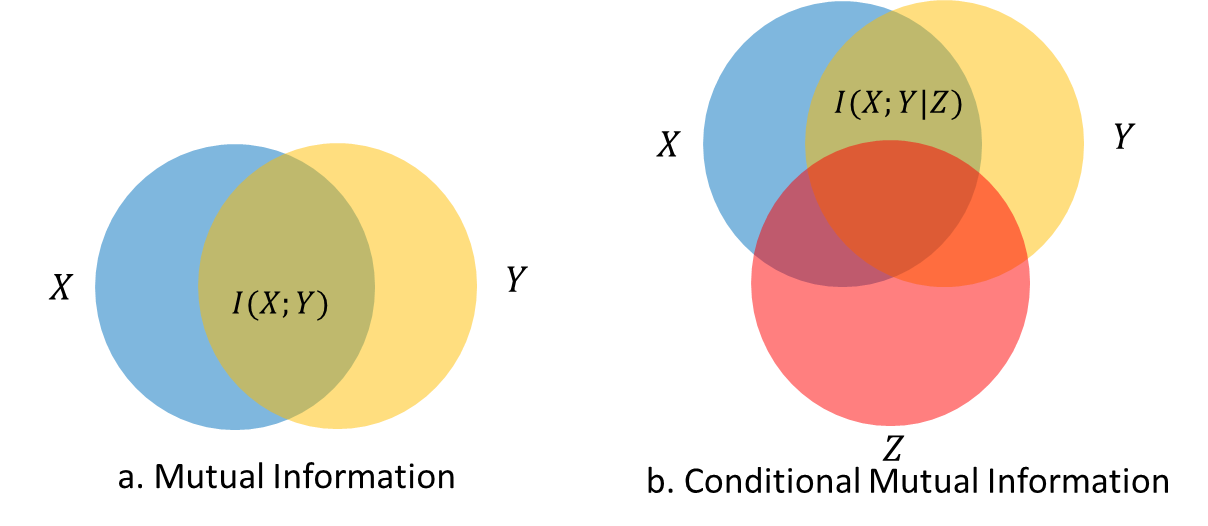
\includegraphics[width=0.8\textwidth]{fig/mutual}
\end{figure}

\begin{equation}\label{info:mutual}
I(X,Y) = H(X) + H(Y) - H(X,Y)
\end{equation}

\begin{equation}
I(X,Y) = H(X) - H(X|Y)
\end{equation}

Mutual information can also be calculated using the probability mass functions directly. In this case we get:

\begin{equation}
I(X,Y) = \sum_{i=1}^{n}\sum_{j=1}^{m}P(x_i, y_j)log_2(\frac{P(x_i, y_j)}{P(x_i)P(y_j)})
\end{equation}
    
While mutual information does show whether there is a relationship or correlation between two variables, it does not give information about the "shape" of the relationship. Making the analogy with figure~\ref{entropy}, mutual information shows how much overlap there is, but it does not explain anything else. Mutual information makes no assumptions of what the distribution of the variables X and Y is like. 

Mutual information, like entropy, is non-negative. Additionally, just like there is conditional entropy, there is also conditional mutual information. Figure~\ref{mutual} shows the conditional mutual information. It refers to the entropy in common between $X$ and $Y$, with the exclusion of $Z$. Conditional mutual information indicates the mutual information given another variable is given:

\begin{equation}
I(X,Y|Z) = \sum_{k=1}^{o}\sum_{i=1}^{n}\sum_{j=1}^{m}P(x_i, y_j, z_k)log_2(\frac{P(x_i, y_j z_k)P(z_k)}{P(x_i, z_k)P(y_j z_k)})
\end{equation}

\section{Multi-Variate Information Theory}\label{multivariate}
In the previous sections, information theory has been observed through a bivariate lens. These methods can be generalised to multivariate variations. When comparing different brain regions, we do not want to restrict ourselves to a bivariate case.

Joint entropy can be easily extended to a multivariate case. In the bivariate case, the joint probability mass function was used and a summation over both random variables was done. The multivariate case simply generalises this equation:

\begin{equation}\label{multivariateentropy}
H(X_1, ..., X_n) = -\sum_{x_1}...\sum_{x_n}P(x_1,...,x_n)log_2(P(x_1,...,x_n))
\end{equation}

Equation~\ref{joint} can also be extended into a multivariate case. In this case, we get:

\begin{equation}
H(X_1, ..., X_n) = -\sum_{k=1}^{n}H(X_k|X_{k-1},...,X_1)
\end{equation}

The multivariate case of conditional entropy becomes:

\begin{equation}\label{condentropy2}
H(Y | X_1, ..., X_n) = H(Y, X_1, ..., X_n) - H(X_1, ..., X_n)
\end{equation}

We can also make a formula to calculate the entropy of multiple variables conditioned on a single variable:

\begin{equation}\label{condentropy}
H(X_1, ..., X_n | Y) = H(Y, X_1, ..., X_n) - H(Y)
\end{equation}

Having extended the different forms of entropy into a multivariate case, we can make a multivariate method for mutual information. The multivariate mutual information becomes a recursive function:

\begin{equation}
I(X_1, ..., X_{n+1}) = I(X_1, ..., X_n) - I(X_1, ..., X_n | X_{n+1})
\end{equation}

The multivariate mutual information can also be decomposed into a som of entropies, which makes it easier to calculate:

\begin{equation}\label{mut}
I(X_1, ..., X_n) = \sum_{T \subseteq \{1,...,n\}} (-1)^{|T|}H(T)
\end{equation}

\begin{equation}\label{condmut}
I(X_1, ..., X_n | Y) = \sum_{T \subseteq \{1,...,n\}} (-1)^{|T|}H(T|Y)
\end{equation}
    
With these formulas, the discussed entropies are formulated in a multivariate way. This specific formulation of multivariate mutual information is also called interaction information in the literature.

Another interesting note is that most equations can be reduced into a sum of (joint) entropies. Equation~\ref{condmut} is formulated as a sum of conditional entropies. But with equation~\ref{condentropy}, we can reduce equation~\ref{condmut} into a sum of entropies without conditional variables. 

Being able to reduce most equations into a sum of entropies becomes a useful ability during the implementation of these equations.

\section{Directed Information}\label{directed-information}

Regular mutual information shows the amount of entropy that is shared between two or more random variables. The mutual information can capture both linear and non-linear relationships. However, mutual information cannot show the information flow between different variables. 

In order to show the information flow, an extension to mutual information has to be made. This extension is called directed information. Directed information uses processes rather than variables. A process $X^n$ is a sequence, a vector of data $X_1,...,X_n$. A time series, by its nature, can be seen as a process.

\begin{equation}
I(X^n \rightarrow Y^n) = \sum^{n}_{i=1}I(X^i, Y_i | Y^{i-1})
\end{equation}

An additional note is that directed information is computationally expensive to compute. Multivariate mutual information has to be calculated $n$ times. This makes computation of long processes slow to compute. 

\section{Continuous Data}\label{binning}
Up until this point, the discussed equations assumed that discrete data was available. However, within the context of neuroscience and the brain, data is almost always continuous in nature. In the case of EEG research, the data comprises of time series of electrical activity.

In the case of this thesis, the data is a time series of source-reconstructed EEG data. In order to compute entropy with continuous data, the data needs to be discretized. There are multiple ways to discretize data:

\begin{itemize}
\item Histogram analysis
\item Correlation analysis
\item Clustering analysis
\item Decision tree analysis
\item Probability modelling
\item Binning
\end{itemize}

These ways utilise different tools, such as histograms, correlation, clustering, decision trees, probability distributions, in order to discretize the data. 

The default choice is to utilise binning. Binning is a relatively simple process that is fast to compute. This is what makes binning attractive. Utilisation of other ways to discretize data is left for future work.

\subsection{Binning}

Binning is the process of putting the continuous data into a predetermined number of bins. In order to avoid adding any kind of noise or bias to the data, every bin should have an equal width. In order to map the continuous data onto the bins, every bin needs to represent a certain interval. The interval of the first bin starts at the minimum value of the continues data. The interval of the last bin ends at the maximum value of the continuous data. The width of the bin is decided by the number of bins. 

\begin{figure}[!htb]
\caption{Binning representation.}
\label{bin-rep}
    \centering
    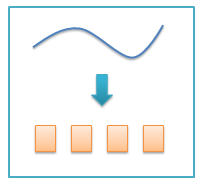
\includegraphics[width=0.5\textwidth]{fig/binning}
\end{figure}

The big question is how many bins should be used to discretize the data. If too little bins are used, information from the continuous data is lost. On the other hand, with a very large amount of bins, each bins will only contain one value. In this case, generality is lost. 

The number of bins used has a large impact on the entropy, so making the correct choice is important. There are multiple ways to make the correct choice. The number of bins can be estimated empirically by plotting the entropy with varying bin sizes. Using this method, the issues that come with a too small or too large bin size can be vizualised. 

There is another, more statistically sound, method for determining the appropriate amount of bins. There is the Freedman-Diaconis rule. This rule states that the optimal amount of bins is related to the interquartile range $Q_x$, the amount of data point $n$ and the minimum $min(x)$ and maximum $max(x)$ elements of the data:

\begin{equation}\label{binequation}
nbins = \frac{max(x) - min(x)}{2Q_xn^{-1/3}}
\end{equation}

\section{Summary}

This chapter provides the necessary mathematical background in order to accomplish the information theoretical analysis of the EEG source-reconstructed data. As explained in section~\ref{multivariate}, most equations can be reduced into a sum of (joint) entropies, which becomes important for the implementation. 

To summarize, the two most important aspects from this chapter are:

\begin{enumerate}
\item Multivariate mutual information
\item Dealing with continuous data
\end{enumerate}

In order to accomplish the analysis from this thesis, the continuous data has to be discretized. More specifically, this thesis uses the binning method in order to discretize the data. The analysis itself focusses on multivariate mutual information. Chapter~\ref{evaluation} will go in depth into the actual analysis that has been done on the data. The binning and the different analysis experiments are described. Chapter~\ref{implementation} goes in depth into the source code that has been developed for the analysis. There are several important aspects to be discussed about the source code. 